\chapter{Introduction}\label{ch:introduction}
The first chapter of the report should be the introduction chapter. The format shown on the first page of this first chapter must be followed in all chapters. The text is double-line spaced. 

Every new paragraph starts with an indentation of one tab space. The font is Regular 12-point Times New Roman and fully justified. The sections are numbered according to the number of Chapter.

\section{Figures and Tables}
There can be several sections within every chapter. The start of every section is indented (similar to paragraph). The number of sections depends upon the text. The sections are numbered according to the chapter number. For example for chapter 1, the sections are 1.1, 1.2, 1.3 and so on. 

The figures and tables are also numbered according to chapter number and will be displayed as same on the list of figures and list of tables, if applicable. You can add an image as shown below and reference it as figure \ref{fig:sample_image}. To reference a figure caption and label are necessary \textbf{and in the same order}. You can read more about inserting images at: \url{https://www.sharelatex.com/learn/Inserting_Images}.

\begin{figure}[ht]
  \centering
  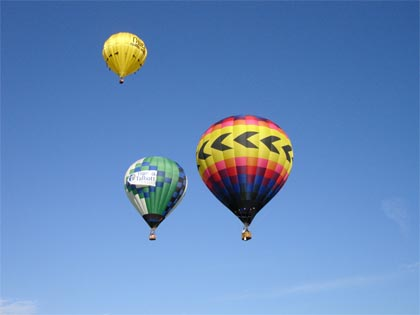
\includegraphics[width=6cm]{images/sample_image.jpeg}
  \caption{Sample Image}
  \label{fig:sample_image}
\end{figure}

A sample table is show below, you can reference it as \ref{tab:sample_table}. Note that the prefix "fig:" in case of figure and "tab:" in case of table isn't required but it's considered as good practice. You can read more about tables at: \url{https://www.sharelatex.com/learn/Tables}.

\begin{table}[ht]
  \centering
  \caption{Sample Table}
  \label{tab:sample_table}
  \begin{tabular}{ |c|c|c|c| } 
    \hline
    col1 & col2 & col3 \\
    \hline
    \multirow{3}{4em}{Multiple row} & cell2 & cell3 \\ 
    & cell5 & cell6 \\ 
    & cell8 & cell9 \\ 
    \hline
  \end{tabular}
\end{table}

\section{References}
You can add a citation in the text using the cite command as \cite{big} or multiple as \cite{big,small}. Citing a paper or journal would automatically add it's details in References section.

\subsection{Subsection within a section}
There can be subsections within the sections. The format of the subsections should be the same as shown in this example. The subsections should also be numbered according to the number of chapter. For example for chapter 1, section 1.1, subsections should be numbered as 1.1.1, 1.1.2 and so on.
